\documentclass[12pt, a4paper]{article}

% --- Font and Language Setup (Requires XeLaTeX compiler) ---
\usepackage[utf8]{inputenc}
\usepackage[T1]{fontenc}
\usepackage{carlito}
\renewcommand{\familydefault}{\sfdefault}

% --- Packages ---
\usepackage{geometry}
\geometry{top=2.5cm, bottom=2.5cm, left=2.5cm, right=2.5cm} % Standard academic margins
\usepackage{graphicx}
\usepackage{amsmath}
\usepackage{amssymb}
\usepackage{subcaption}
\usepackage{titlesec}
\usepackage[hidelinks]{hyperref}
\usepackage{xcolor}
\usepackage{listings}

% --- Python Code Formatting Setup ---
\definecolor{codegreen}{rgb}{0,0.6,0}
\definecolor{codegray}{rgb}{0.5,0.5,0.5}
\definecolor{codepurple}{rgb}{0.58,0,0.82}
\definecolor{backcolour}{rgb}{0.95,0.95,0.92}

\lstdefinestyle{mystyle}{
    backgroundcolor=\color{backcolour},   
    commentstyle=\color{codegreen},
    keywordstyle=\color{magenta},
    numberstyle=\tiny\color{codegray},
    stringstyle=\color{codepurple},
    basicstyle=\ttfamily\footnotesize,
    breakatwhitespace=false,         
    breaklines=true,                 
    captionpos=b,                    
    keepspaces=true,                 
    numbers=left,                    
    numbersep=5pt,                  
    showspaces=false,                
    showstringspaces=false,
    showtabs=false,                  
    tabsize=2
}
\lstset{style=mystyle}

% --- Document Info ---
\title{
    \Large \textbf{MATPMD4: Optimisation Assignment}
}
\author{Student ID: 3539054}
\date{April 8, 2026}

\begin{document}

\maketitle

\section{Maximising a Function}

\subsection{Problem Definition}

The primary objective is to find the global maximum of the continuous function $f(x, y, z)$, subject to strict boundary constraints.

\vspace{0.5cm}

\hspace{-1.5em}\textbf{Objective Function:}

\vspace{0.25cm}

\hspace{-1.5em}Maximise $f(x, y, z)$ where:
\begin{align*}
f(x, y, z) &= -e^{-(x - 0.55z)^2} \cos(81(x + z + 0.12y)) + \sin(44(y + 0.03(x - z))) \\
&\quad - \cos(69 \sin(xz + 0.07y)) - \sin(1.32(x - z)) - 0.32(z + 0.22xz)^2 e^{\sin(63(z - x))} \\
&\quad + \cos(77x) + \sin(71z) - e^{-y^2} \cos(75y) + \sin(43y) + \cos(73y) + 0.05(x^2 + y^2 + z^2)
\end{align*}

\vspace{0.5cm}

\hspace{-1.5em}\textbf{Constraints:}
\begin{align*}
0 &\le x \le 5 \\
0 &\le y \le 5 \\
0 &\le z \le 5
\end{align*}

\vspace{0.5cm}

\hspace{-1.5em}\textbf{Landscape Visualisation:}

\vspace{0.25cm}

Since the objective function relies on three independent variables ($x, y, z$), the complete search space is 4-dimensional and impossible to plot. To visualise the terrain, take a \textit{slice} of the space by holding one variable constant. Figure~\ref{fig:3d-2d-1} fixes $z = 0.199$ and zooms into a narrow, $0.5 \times 0.5$ window for $x$ and $y$. Looking closely at this small area shows its real complexity. The surface is full of sharp peaks and steep valleys caused by overlapping trigonometric terms. This multimodal landscape explains why simple gradient-based methods would easily get stuck. It also shows why we need a strong random algorithm to explore this space effectively.

\newpage

\begin{figure}[t]
    \centering
    \begin{subfigure}[t]{0.5\linewidth}
    \centering
        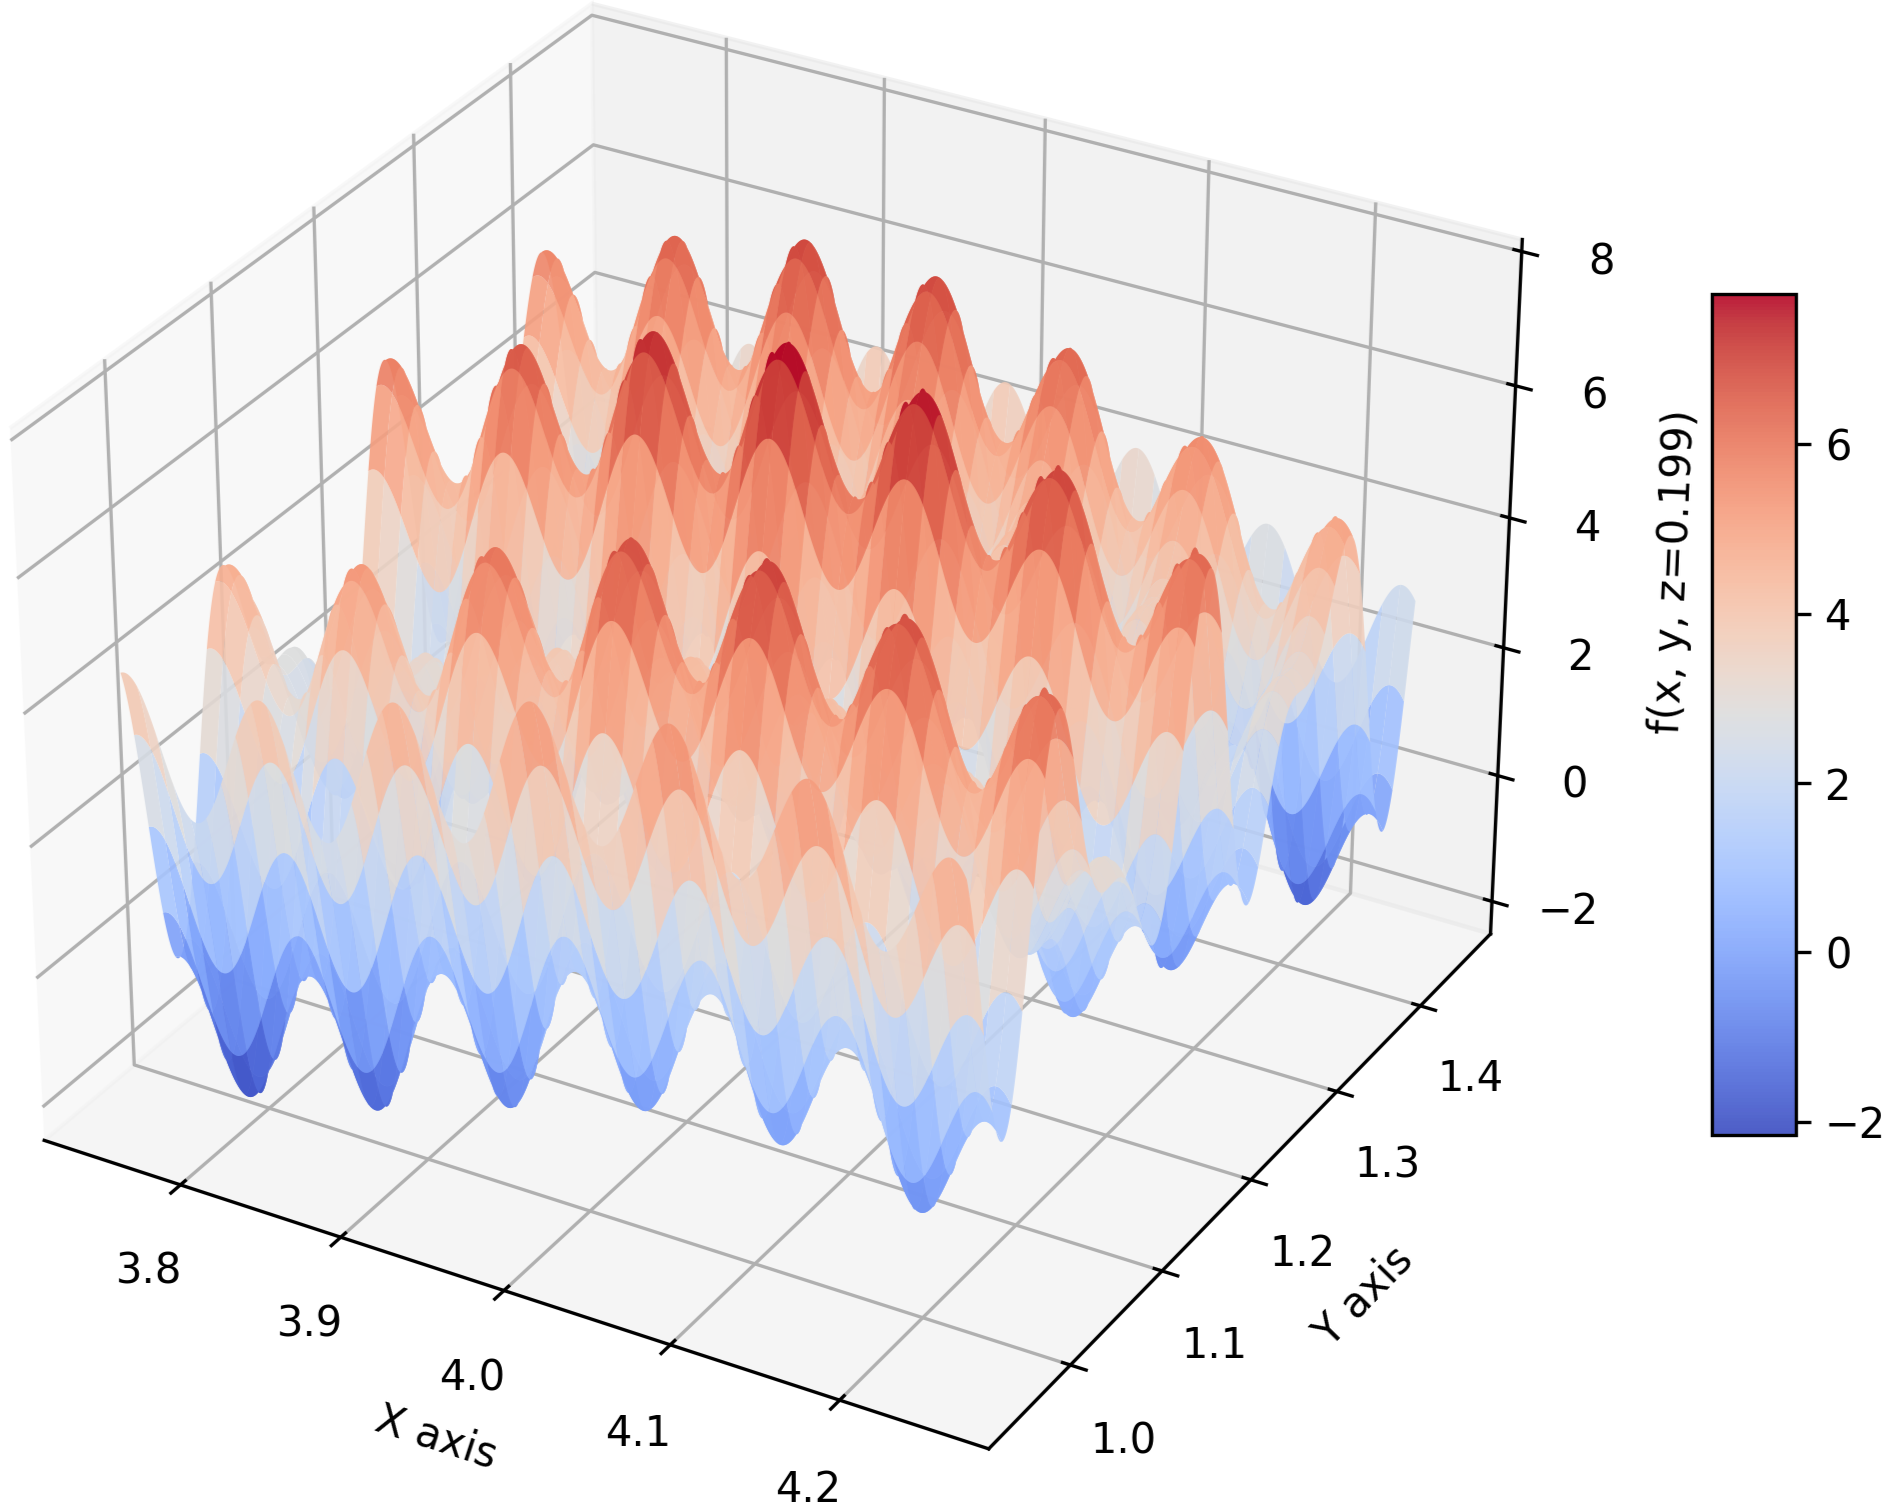
\includegraphics[width=1\linewidth]{images/landscape_3d_surface.png}
        \caption{3D surface plot}
        \label{fig:3d-1}
    \end{subfigure}
    \hfill
    \begin{subfigure}[t]{0.49\linewidth}
    \centering
        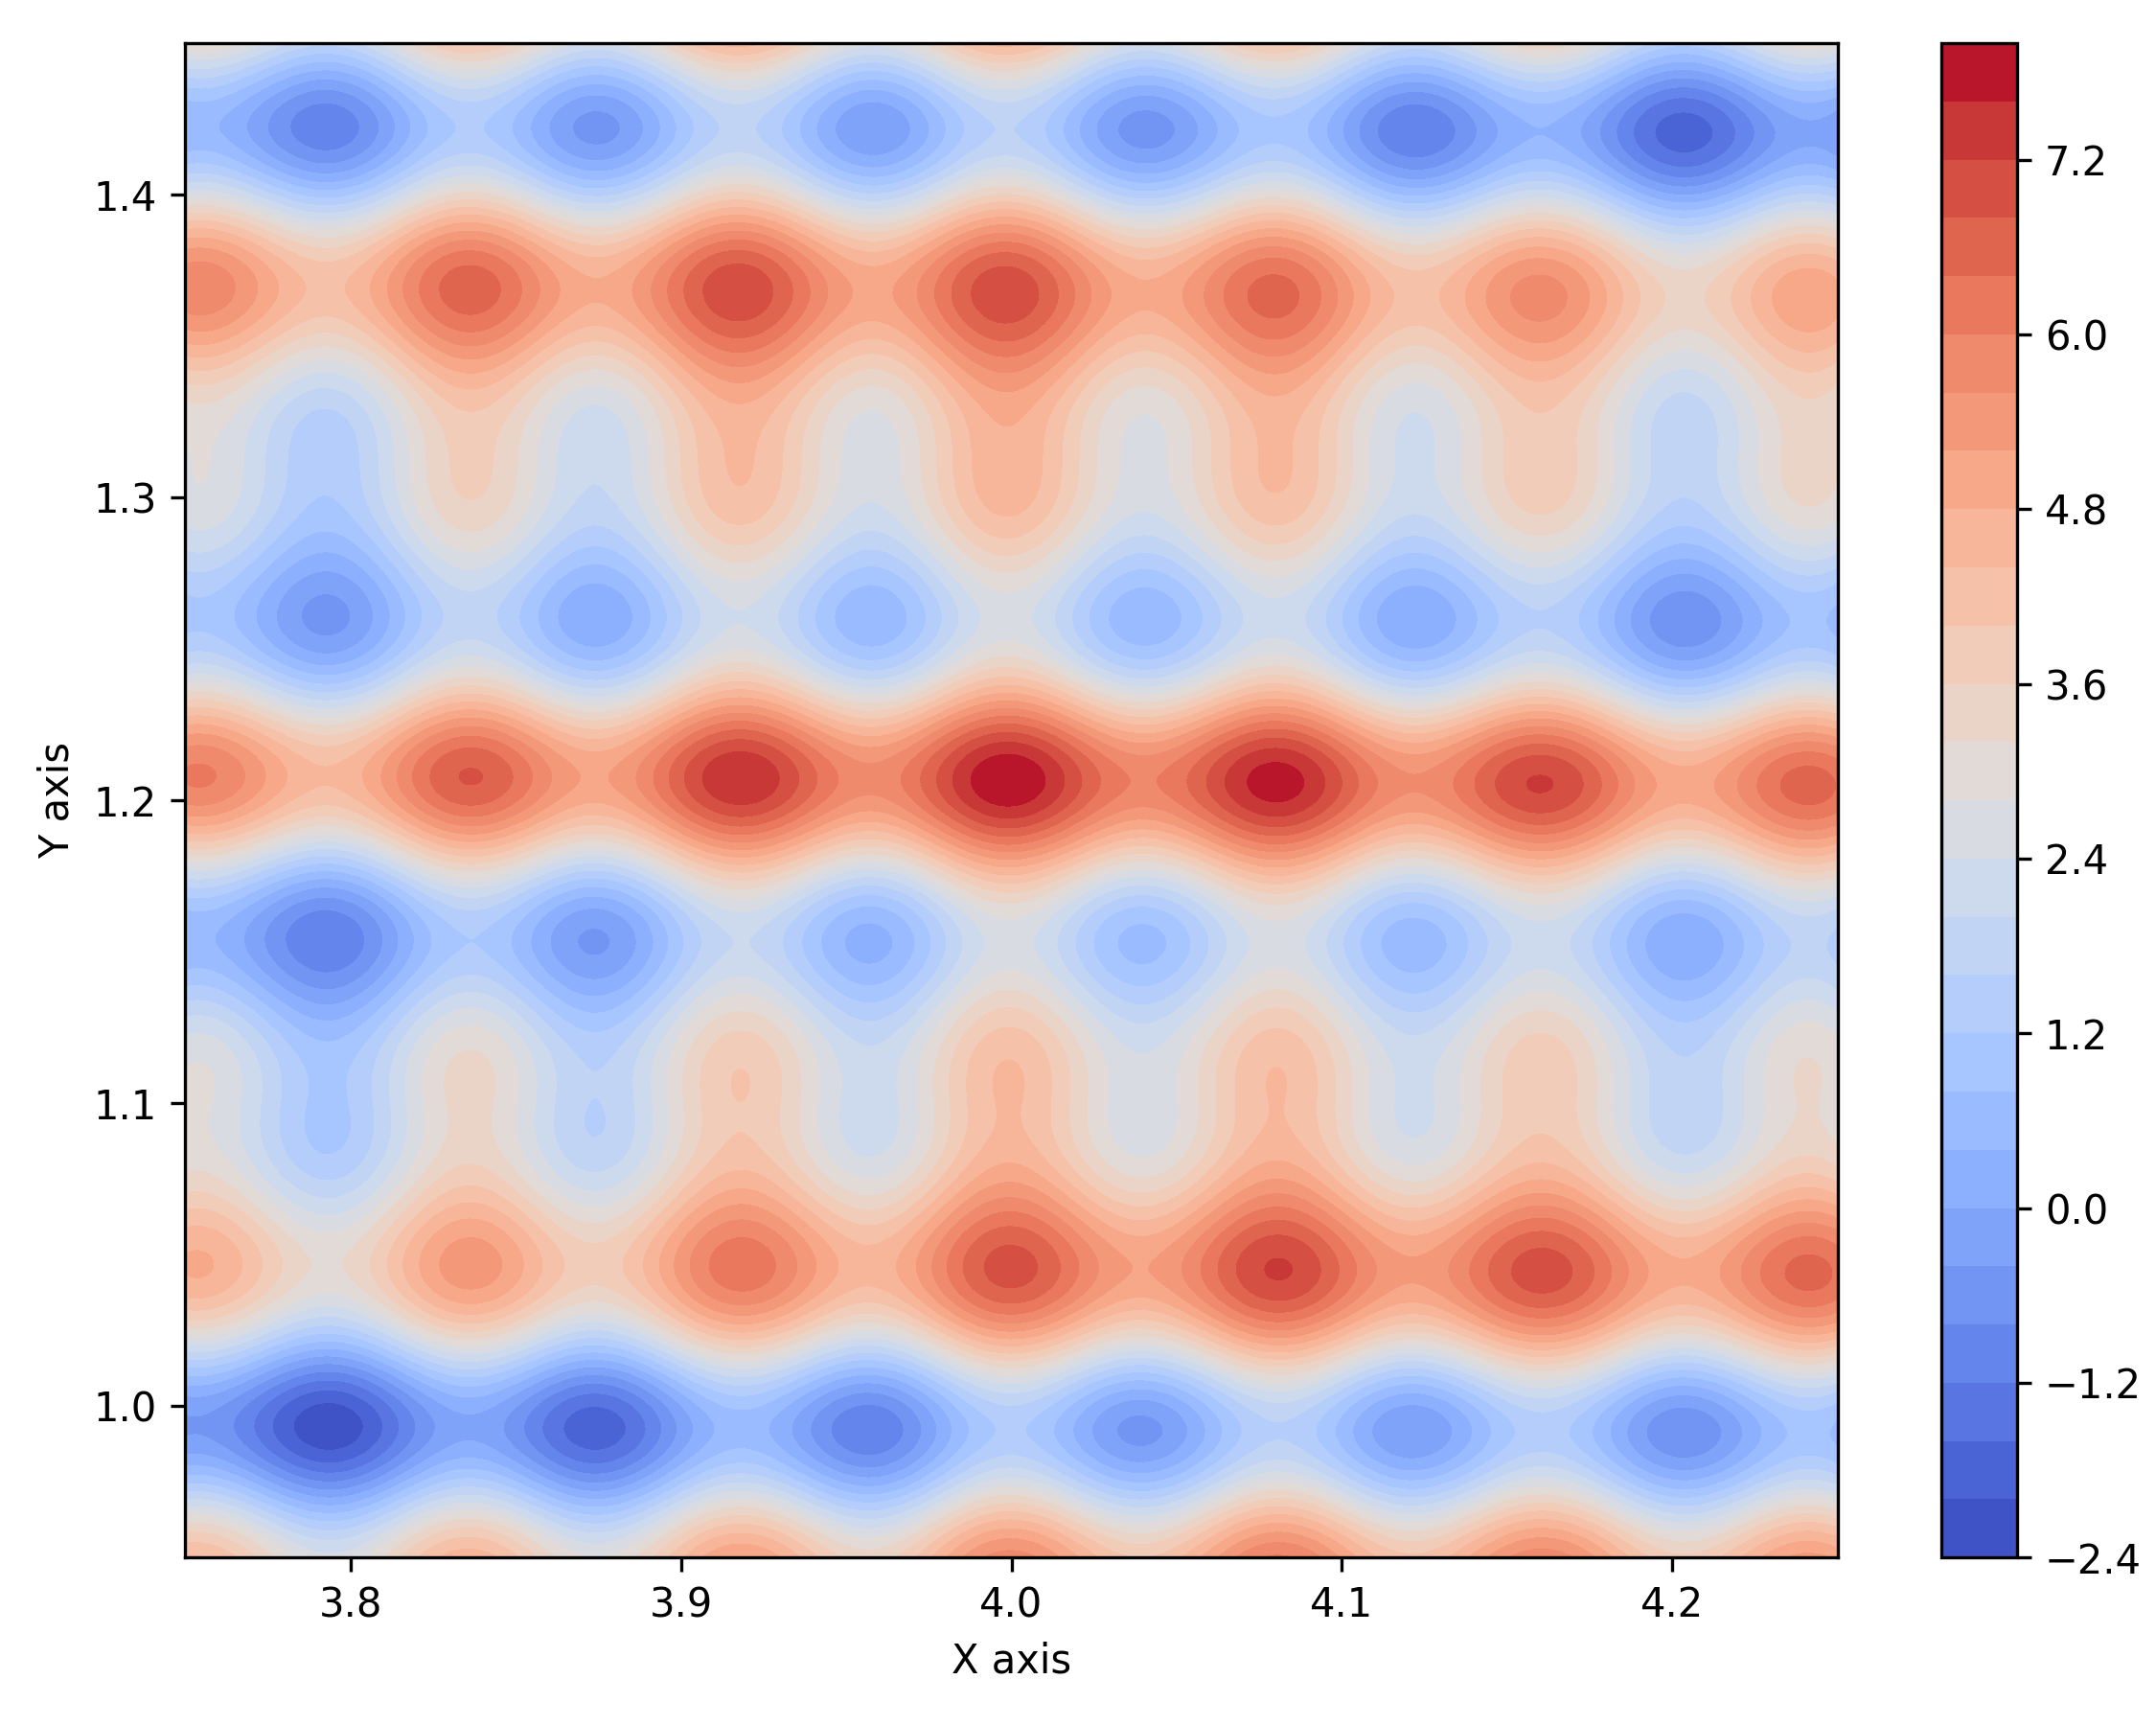
\includegraphics[width=1\linewidth]{images/landscape_2d_contour.png}
        \caption{2D contour map}
        \label{fig:2d-1}
    \end{subfigure}
    \caption{Visualisations of the objective function's fitness landscape at the fixed slice $z = 0.199$. The view is zoomed in at $3.75 \leq x \leq 4.25$ and $0.95 \leq y \leq 1.45$}
    \label{fig:3d-2d-1}
\end{figure}

\vspace{0.5cm}

\subsection{Algorithm Selection and Justification}

\quad Knowing that the objective function is complicated, a robust search strategy is needed. Methods like Hill Climbing or basic Simulated Annealing only keep one solution and try to make it better step by step. In a topography with many false peaks, these single-state methods often get stuck at a local maximum and cannot escape \cite{Luke2013Metaheuristics}. To overcome this, a \textbf{population-based method} is better. Population-based algorithms keep a variety of possible solutions. This allows exploration of different areas at the same time. By evaluating many options together, the risk of settling on a local maximum is reduced.

\vspace{0.5cm}

To solve this specific problem, a $(\mu + \lambda)$ \textbf{Evolution Strategy} (\textit{ES}) was selected. \textit{ES} is a population-based metaheuristic explicitly designed for continuous, real-valued $(\mathbb{R})$ optimisation. It was preferred because:

\begin{itemize}
    \item \textbf{Real-Valued $(\mathbb{R})$ Population:} A parent population of size $\mu$ is maintained. Since the algorithm's parameters are real numbers, it can work with the coordinates $(x, y, z)$.

    \item \textbf{Gaussian Mutation:} Parents produce $\lambda$ offspring by adding random noise to their coordinates. This noise follows a normal distribution, which helps balance two approaches: making small, frequent adjustments to climb local peaks (\textit{exploitation}) and taking occasional large jumps to escape traps (\textit{exploration}).

    \item \textbf{Selection (Elitism):} The $\mu$ parents and $\lambda$ offspring are combined, and the fittest $\mu$ individuals survive to the next generation. This $(\mu + \lambda)$ selection makes sure that the best solutions are preserved.
\end{itemize}

\newpage

\subsection{Algorithm Implementation and Results}

\vspace{0.5cm}

\textbf{Constraint Handling:}

\vspace{0.25cm}

To enforce the strict boundary conditions $(x, y, z \in [0, 5])$, a clamping function was implemented. During reproduction, if a mutation moved a child's coordinate outside the allowed range, it was adjusted back to the closest valid boundary.

\vspace{0.5cm}

\noindent\begin{minipage}{1\linewidth}
    \begin{lstlisting}[language=Python, caption=Constraint Handling and Mutation Logic, label=lst:constraint_and_mutation_1]
def clamp(value, min_bound=0.0, max_bound=5.0):
    return max(min_bound, min(value, max_bound))

# ... [Code skipped: inside the run_evolution_strategy loop] ...

# Gaussian mutation
child = {
    'x': clamp(parent['x'] + random.gauss(0, mutation_step_size)),
    'y': clamp(parent['y'] + random.gauss(0, mutation_step_size)),
    'z': clamp(parent['z'] + random.gauss(0, mutation_step_size))
}
    \end{lstlisting}
\end{minipage}

\vspace{0.5cm}

\hspace{-1.5em}\textbf{Hyperparameter Optimisation:}

\vspace{0.25cm}

Stochastic algorithms use randomness, so running the program only once doesn't ensure the best result. To find the most reliable settings, different combinations of parent sizes ($\mu$) and offspring sizes ($\lambda$) were tested. The tests showed that using a small group of 10 parents to create a large pool of 300 offspring ($\mu=10, \lambda=300$) gave the best results. This approach allowed the algorithm to quickly get rid of poor options while still exploring nearby peaks effectively.

\vspace{0.5cm}

\noindent\begin{minipage}{1\linewidth}
    \begin{lstlisting}[language=Python, caption=Automated grid search implementation for hyperparameter optimisation across varying parent $(\mu)$ and offspring $(\lambda)$ population sizes., label=lst:hyperparameter_1]
mu_options = [10, 30, 50]
lambda_options = [50, 150, 300]
trials_per_combo = 3

for mu, lambda_ in itertools.product(mu_options, lambda_options):
    for trial in range(trials_per_combo):
        result = run_evolution_strategy(mu, lambda_)
        if result['fitness'] > best_overall['fitness']:
            best_overall = result
            best_params = {'mu': mu, 'lambda': lambda_}
    \end{lstlisting}
\end{minipage}

\vspace{0.5cm}

\hspace{-1.5em}\textbf{Final Results:}

\vspace{0.25cm}

\hspace{-1.5em}Using the optimised parameters, the algorithm discovered the following global maximum:

\begin{itemize}
    \item \textbf{Optimal Fitness:} $7.952102$

    \item \textbf{Coordinates:} $x=4.000815, y=1.204875, z=0.200288$
\end{itemize}

\newpage

\section{Distribution Network}

\subsection{Problem Definition}

\quad The scenario involves a Multi-Depot Heterogeneous Fleet Vehicle Routing Problem (\textit{MDHFVRP}) on a 2D plane. To speed up mathematical calculations during the algorithm's process, the physical coordinates $(x_i, y_i)$ of the two warehouses $(W1, W2)$ and the $23$ stores were reorganised into a \texttt{numpy} array.

\vspace{0.5cm}

First, a $25 \times 25$ \textbf{Euclidean distance matrix} was generated, where the distance between any two nodes is $d_{ij} = \sqrt{(x_i - x_j)^2 + (y_i - y_j)^2}$. By calculating these distances in advance, the routing algorithm can quickly look them up in constant time, rather than having to recalculate the distances repeatedly during the simulation.

\vspace{0.5cm}

Secondly, the coordinates were transformed to find the \textbf{polar angle} $(\theta)$ of each store relative to both $W1$ and $W2$ (Figure~\ref{fig:supermarket_network}). By doing this before starting the algorithm, we set the stage for using an \textit{angular sweep} heuristic. This heuristic avoids extreme angle differences, helping the vehicles to create more efficient routes instead of zig-zagging.

\begin{figure}[h!]
    \centering
    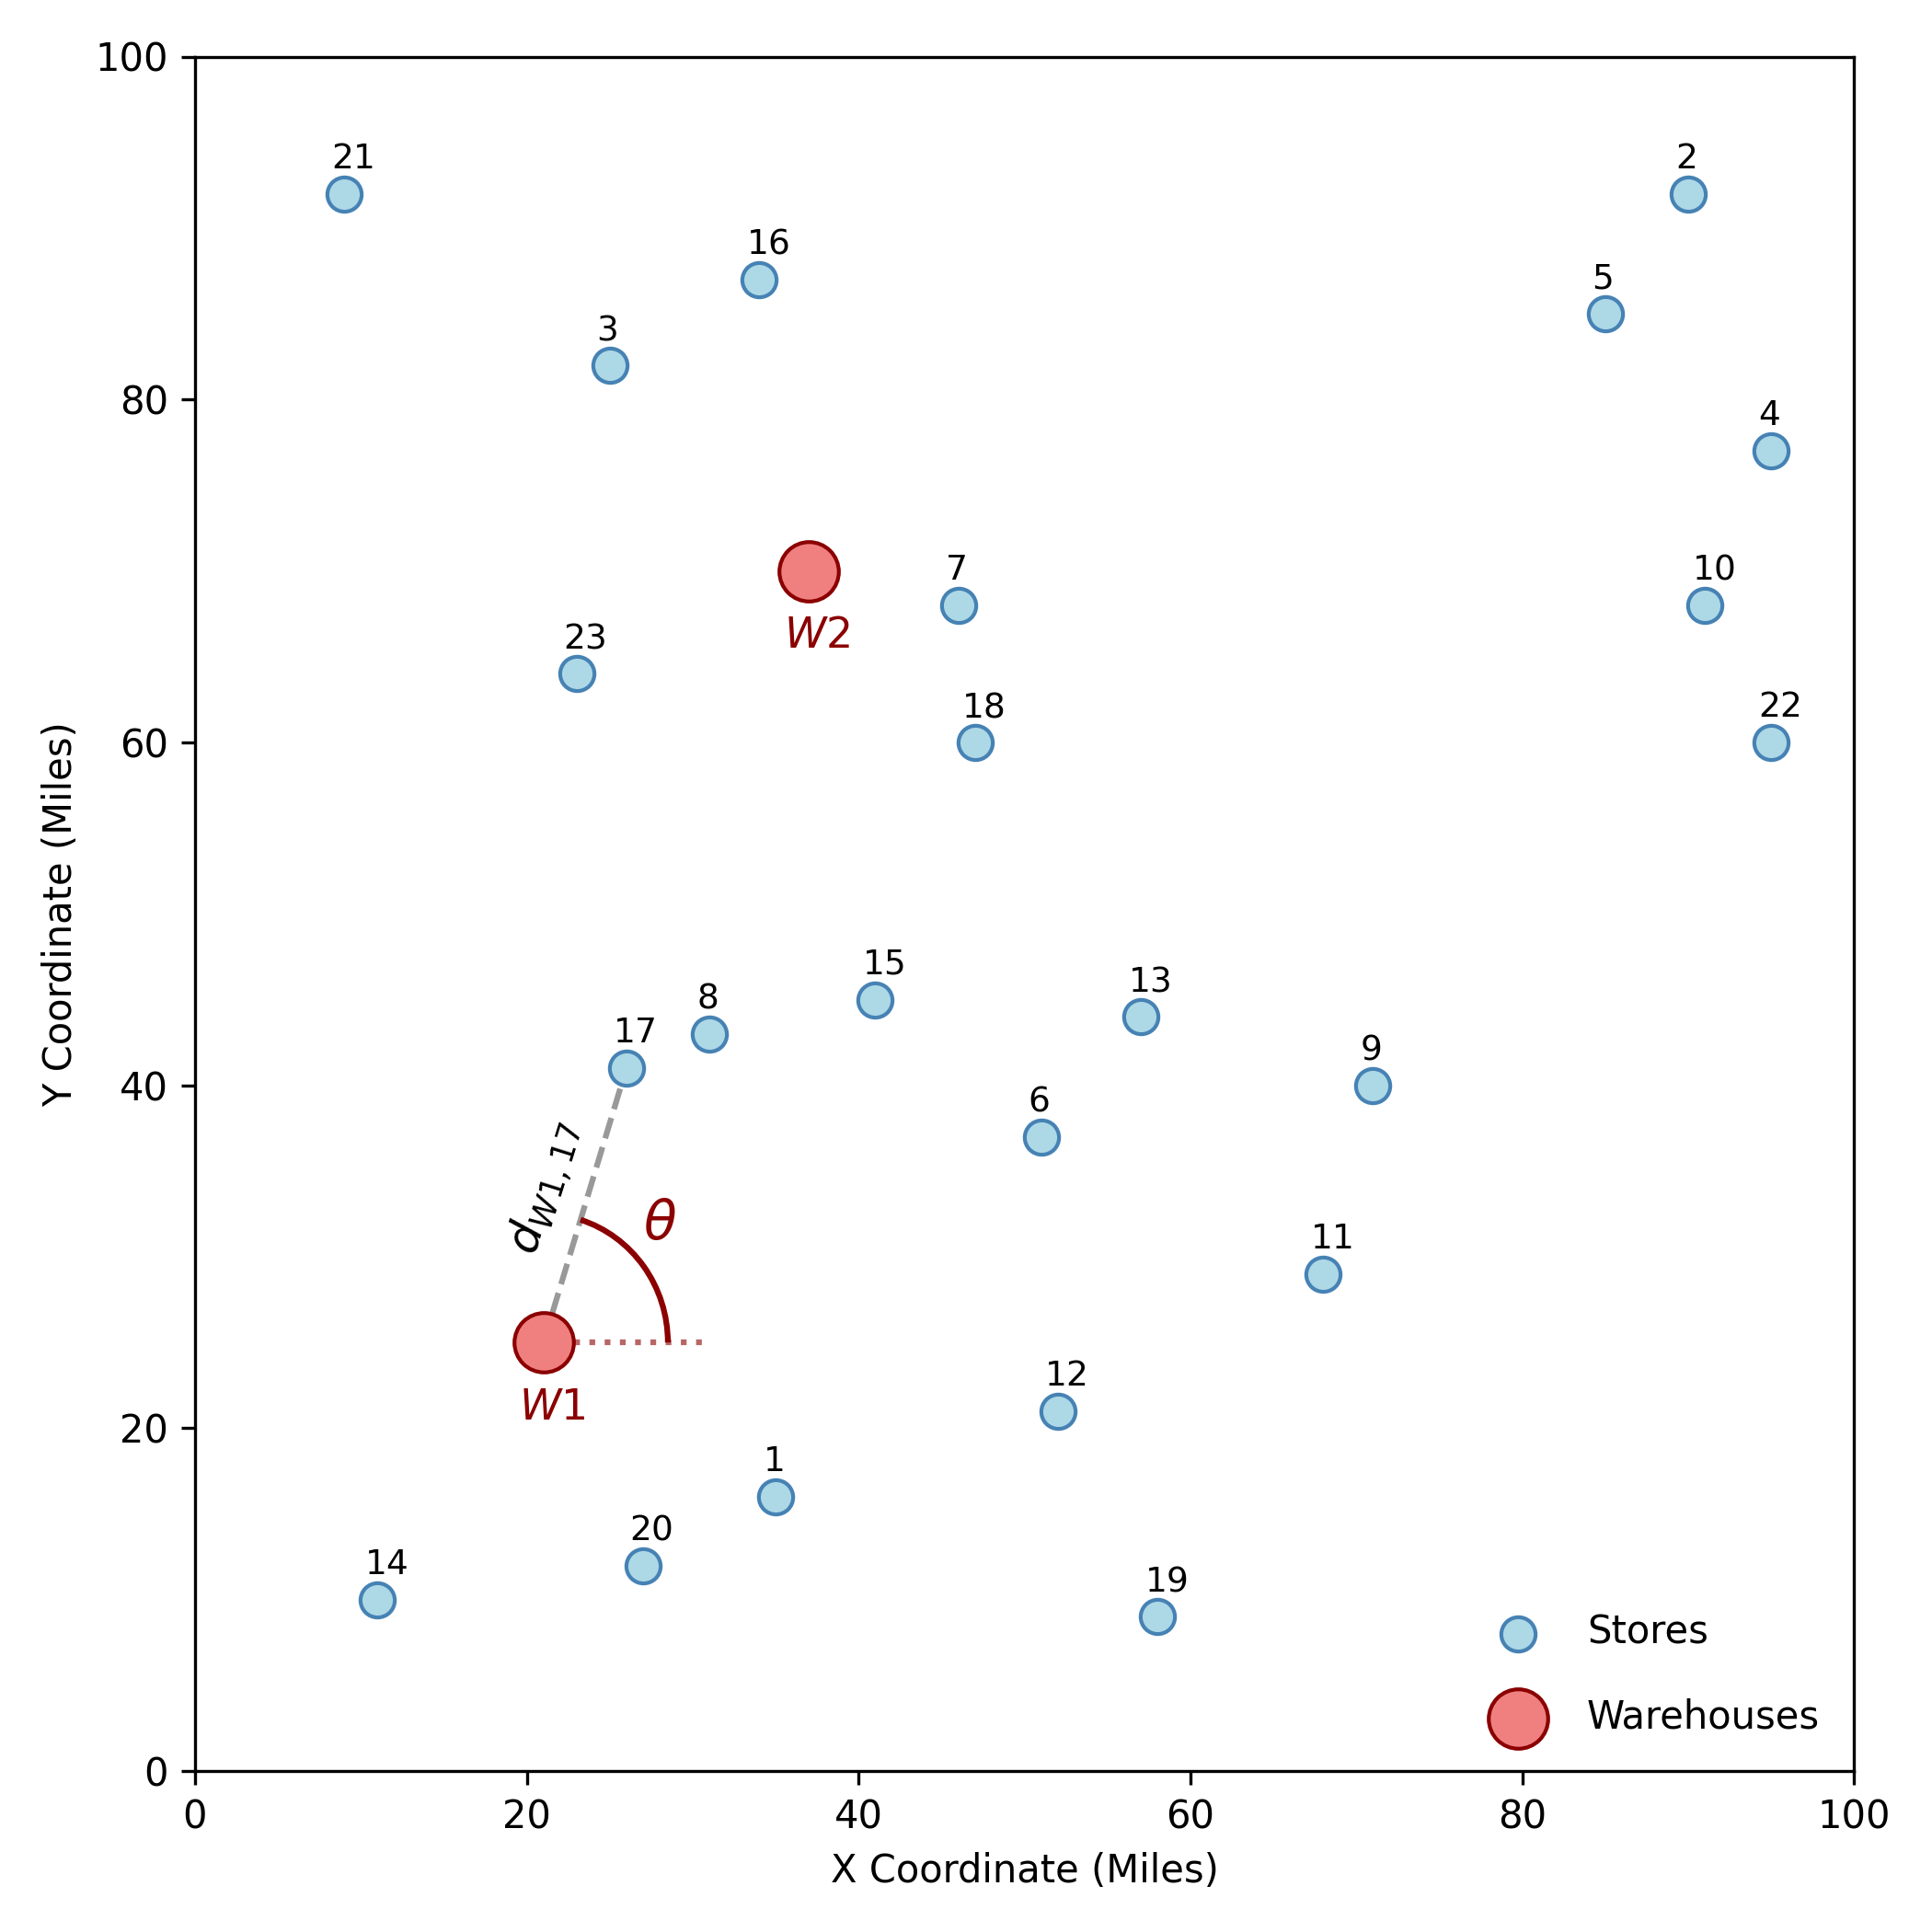
\includegraphics[width=0.85\linewidth]{images/supermarket_network.png}
    \caption{The supermarket distribution network featuring $23$ stores and $2$ warehouses $(W1, W2)$. It illustrates the extraction of Euclidean distance $(d_{W1, 17})$ and polar angle $(\theta)$.}
    \label{fig:supermarket_network}
\end{figure}

\subsection{Algorithm Selection and Justification}

\quad To solve this routing problem, both \textbf{Genetic Algorithms} (\textit{GA}) and \textbf{Ant Colony Optimisation} (\textit{ACO}) were considered. \textit{GAs} can find good solutions, but they struggle with routing problems that have strict rules. Research shows that using standard genetic crossover on a routing sequence often creates invalid routes, such as visiting one store multiple times while missing others \cite{Luke2013Metaheuristics}. Although special techniques like Partially Mapped Crossover (PMX) can help avoid duplication, mixing routes makes it hard to maintain strict limits on vehicle capacities (5 stores for Vans, 18 for Lorries). As a result, a \textit{GA} would need costly repair processes in every generation to fix overloaded vehicles.

\vspace{0.5cm}

\textbf{\textit{ACO} was chosen} as the best architecture for this task. It was originally designed for routing networks. \textit{ACO} works by having agents (\textit{ants}) build solutions step-by-step. These ants are guided by how desirable a path is and the pheromone trails they leave behind \cite{Luke2013Metaheuristics}. This step-by-step process allows \textit{ACO} to handle strict rules naturally instead of fixing them later. As an ant moves through the network, it keeps track of its load. If a vehicle reaches its maximum capacity, the routing system automatically directs it to return to the depot to finish the route. By following the actual limits of the vehicles and avoiding complex fixes, \textit{ACO} offers a much simpler and more reliable way to solve this optimisation problem.

\vspace{0.5cm}

\subsection{Heuristic Implementations}

\quad To optimise the routing patterns, the standard \textit{ACO} heuristic was replaced with a custom evaluation function combining \textbf{Clarke-Wright distance savings} with an \textbf{angular sweep penalty}. Rather than simply prioritising the nearest unvisited node, the algorithm calculates the distance saved by combining two stores into a single route relative to the active warehouse.

$$S_{ij} = d_{w,i} + d_{w,j} - d_{i,j}$$

\hspace{-1.5em}To prevent the generation of disjointed, \textit{zig-zagging} routes, this savings value is penalised by the absolute angular difference $(\Delta\theta)$ in radians between the two nodes. The final desirability is calculated as:

$$S_{ij} / (1 + \Delta\theta)$$

\hspace{-1.5em}The addition of $1.0$ to the denominator prevents a \texttt{DivisionByZero} error if two candidate stores share an identical polar trajectory from the warehouse.

\vspace{0.5cm}

Furthermore, to ensure the generated routing sequences remained geometrically sound, a \textbf{2-Opt} local search mechanism was implemented. A completed vehicle route is represented as a one-dimensional array of indices beginning and terminating at the designated warehouse. For example, $[23, 15, 6, 8, 23]$ denotes a vehicle leaving Warehouse 1, visiting three stores, and returning. Due to the probabilistic nature of the ant agents, initial routes may contain intersecting paths. The \textbf{Triangle Inequality} implies that intersecting lines on a 2D Euclidean plane will produce a longer total distance than a non-intersecting configuration. The 2-Opt function scans the route array for any two crossing edges where reversing the internal sub-route (e.g., flipping the visitation order from $[15, 6]$ to $[6, 15]$) yields a shorter combined distance. This iterative untangling ensures the \textit{pheromone} matrix is updated with optimal, non-intersecting sub-routes.

\subsection{Algorithm Implementation and Results}

\vspace{0.5cm}

\textbf{Constraint Handling:}

\vspace{0.25cm}

\textit{Ant Colony Optimisation} uses a constructive approach, allowing it to manage different vehicle capacities (Vans = 5 stores, Lorries = 18 stores) during route planning,  rather than relying on retroactive repair functions. The algorithm keeps track of each route's payload. If a path reaches the maximum capacity of a Lorry, the system forces the route back to the warehouse.

\vspace{0.5cm}

\hspace{-1.5em}To ensure accuracy in both design and function, the architecture clearly separates the algorithmic agents (\textit{ants}) from the physical fleet (\textit{vehicles}):

\begin{itemize}
    \item \textbf{Ant (The Algorithmic Agent):} An ant does not represent a single vehicle; rather, it acts as a \textit{fleet manager} constructing a complete daily strategy. A single ant will sequentially deploy and route multiple vehicles until all 23 stores are serviced, at which point it evaluates the total combined cost of the entire fleet to inform its \textit{pheromone} deposit.

    \item \textbf{Vehicle (The Capacitated Sub-Route):} The Vans and Lorries represent the physical, constrained resources allocated by the ant. A vehicle's route is simply a single, closed loop originating from a warehouse, visiting a limited subset of stores, and returning, functioning as one isolated component of the ant's overarching master plan.
\end{itemize}

\noindent\begin{minipage}{1\linewidth}
    \begin{lstlisting}[language=Python, caption=Agent logic for handling vehicle constraints without the need for retroactive route repair., label=lst:constraint_2]
# Constructive constraint enforcement during sub-route generation
if len(route) - 1 == LORRY_CAPACITY:
    valid_nodes = [warehouse] # Forces immediate return to warehouse to close the sub-route
    \end{lstlisting}
\end{minipage}

\vspace{0.5cm}

\textbf{Hyperparameter Selection:}

\vspace{0.25cm}

The stability of the optimal solution depends on carefully adjusting the ACO hyperparameters. The heuristic importance $(\beta)$ was set much higher than the pheromone importance $(\alpha)$ to make sure the ants focus on the custom \textit{Clarke-Wright} and \textit{angular sweep} heuristic instead of blind swarm behaviours in the early stages. Additionally, a test showed that increasing the colony to $50$ ants led to \textit{Incremental Stagnation}. This happened because too many overlapping, slightly improved pheromone trails confused the swarm. A colony of $40$ ants with a $10\%$ evaporation rate worked well for Elitist Updates.

\vspace{0.25cm}

\noindent\begin{minipage}{1\linewidth}
    \begin{lstlisting}[language=Python, caption=The optimal hyperparameters to prioritise heuristics and prevent incremental stagnation within the swarm., label=lst:hyperparameter_2]
num_ants = 40
generations = 100
# Importance of pheromones
alpha = 1.0
# Importance of the heuristic (Set high to respect the Savings/Sweep)
beta = 3.0
evaporation = 0.1  # Pheromone decay rate
    \end{lstlisting}
\end{minipage}

\textbf{Final Results:}

\vspace{0.25cm}

The optimisation framework achieved a minimum daily distribution cost of \pounds$1118.29$. The algorithm capitalised on the efficiency of \textit{Stem Miles} by fully maximising a single Lorry (\pounds$3.00$/mile) from Warehouse $1$ to sweep the bulk of the network, dispatching only a single Van (\pounds$2.00$/mile) from Warehouse $2$ to clear the remaining outlier cluster.

\vspace{0.5cm}

\hspace{-1.5em}Optimised Configuration (Figure~\ref{fig:supermarket_solution}):

\begin{itemize}
    \item \textbf{Total Daily Cost:} \pounds$1118.29$

    \item \textbf{Route 1 (Lorry,} \pounds$903.51$\textbf{):}
    $$\begin{aligned}
        W1 &\rightarrow 17 \rightarrow 8 \rightarrow 15 \rightarrow 6 \rightarrow 13 \rightarrow 18 \rightarrow 5 \rightarrow 2 \rightarrow 4 \rightarrow 10 \rightarrow 22 \\
        &\rightarrow 9 \rightarrow 11 \rightarrow 19 \rightarrow 12 \rightarrow 1 \rightarrow 20 \rightarrow 14 \rightarrow W1
    \end{aligned}$$

    \item \textbf{Route 2 (Van,} \pounds$214.78$\textbf{):}
    $\begin{aligned}
        W2 \rightarrow 7 \rightarrow 16 \rightarrow 3 \rightarrow 21 \rightarrow 23 \rightarrow W2
    \end{aligned}$
\end{itemize}

\begin{figure}[h!]
    \centering
    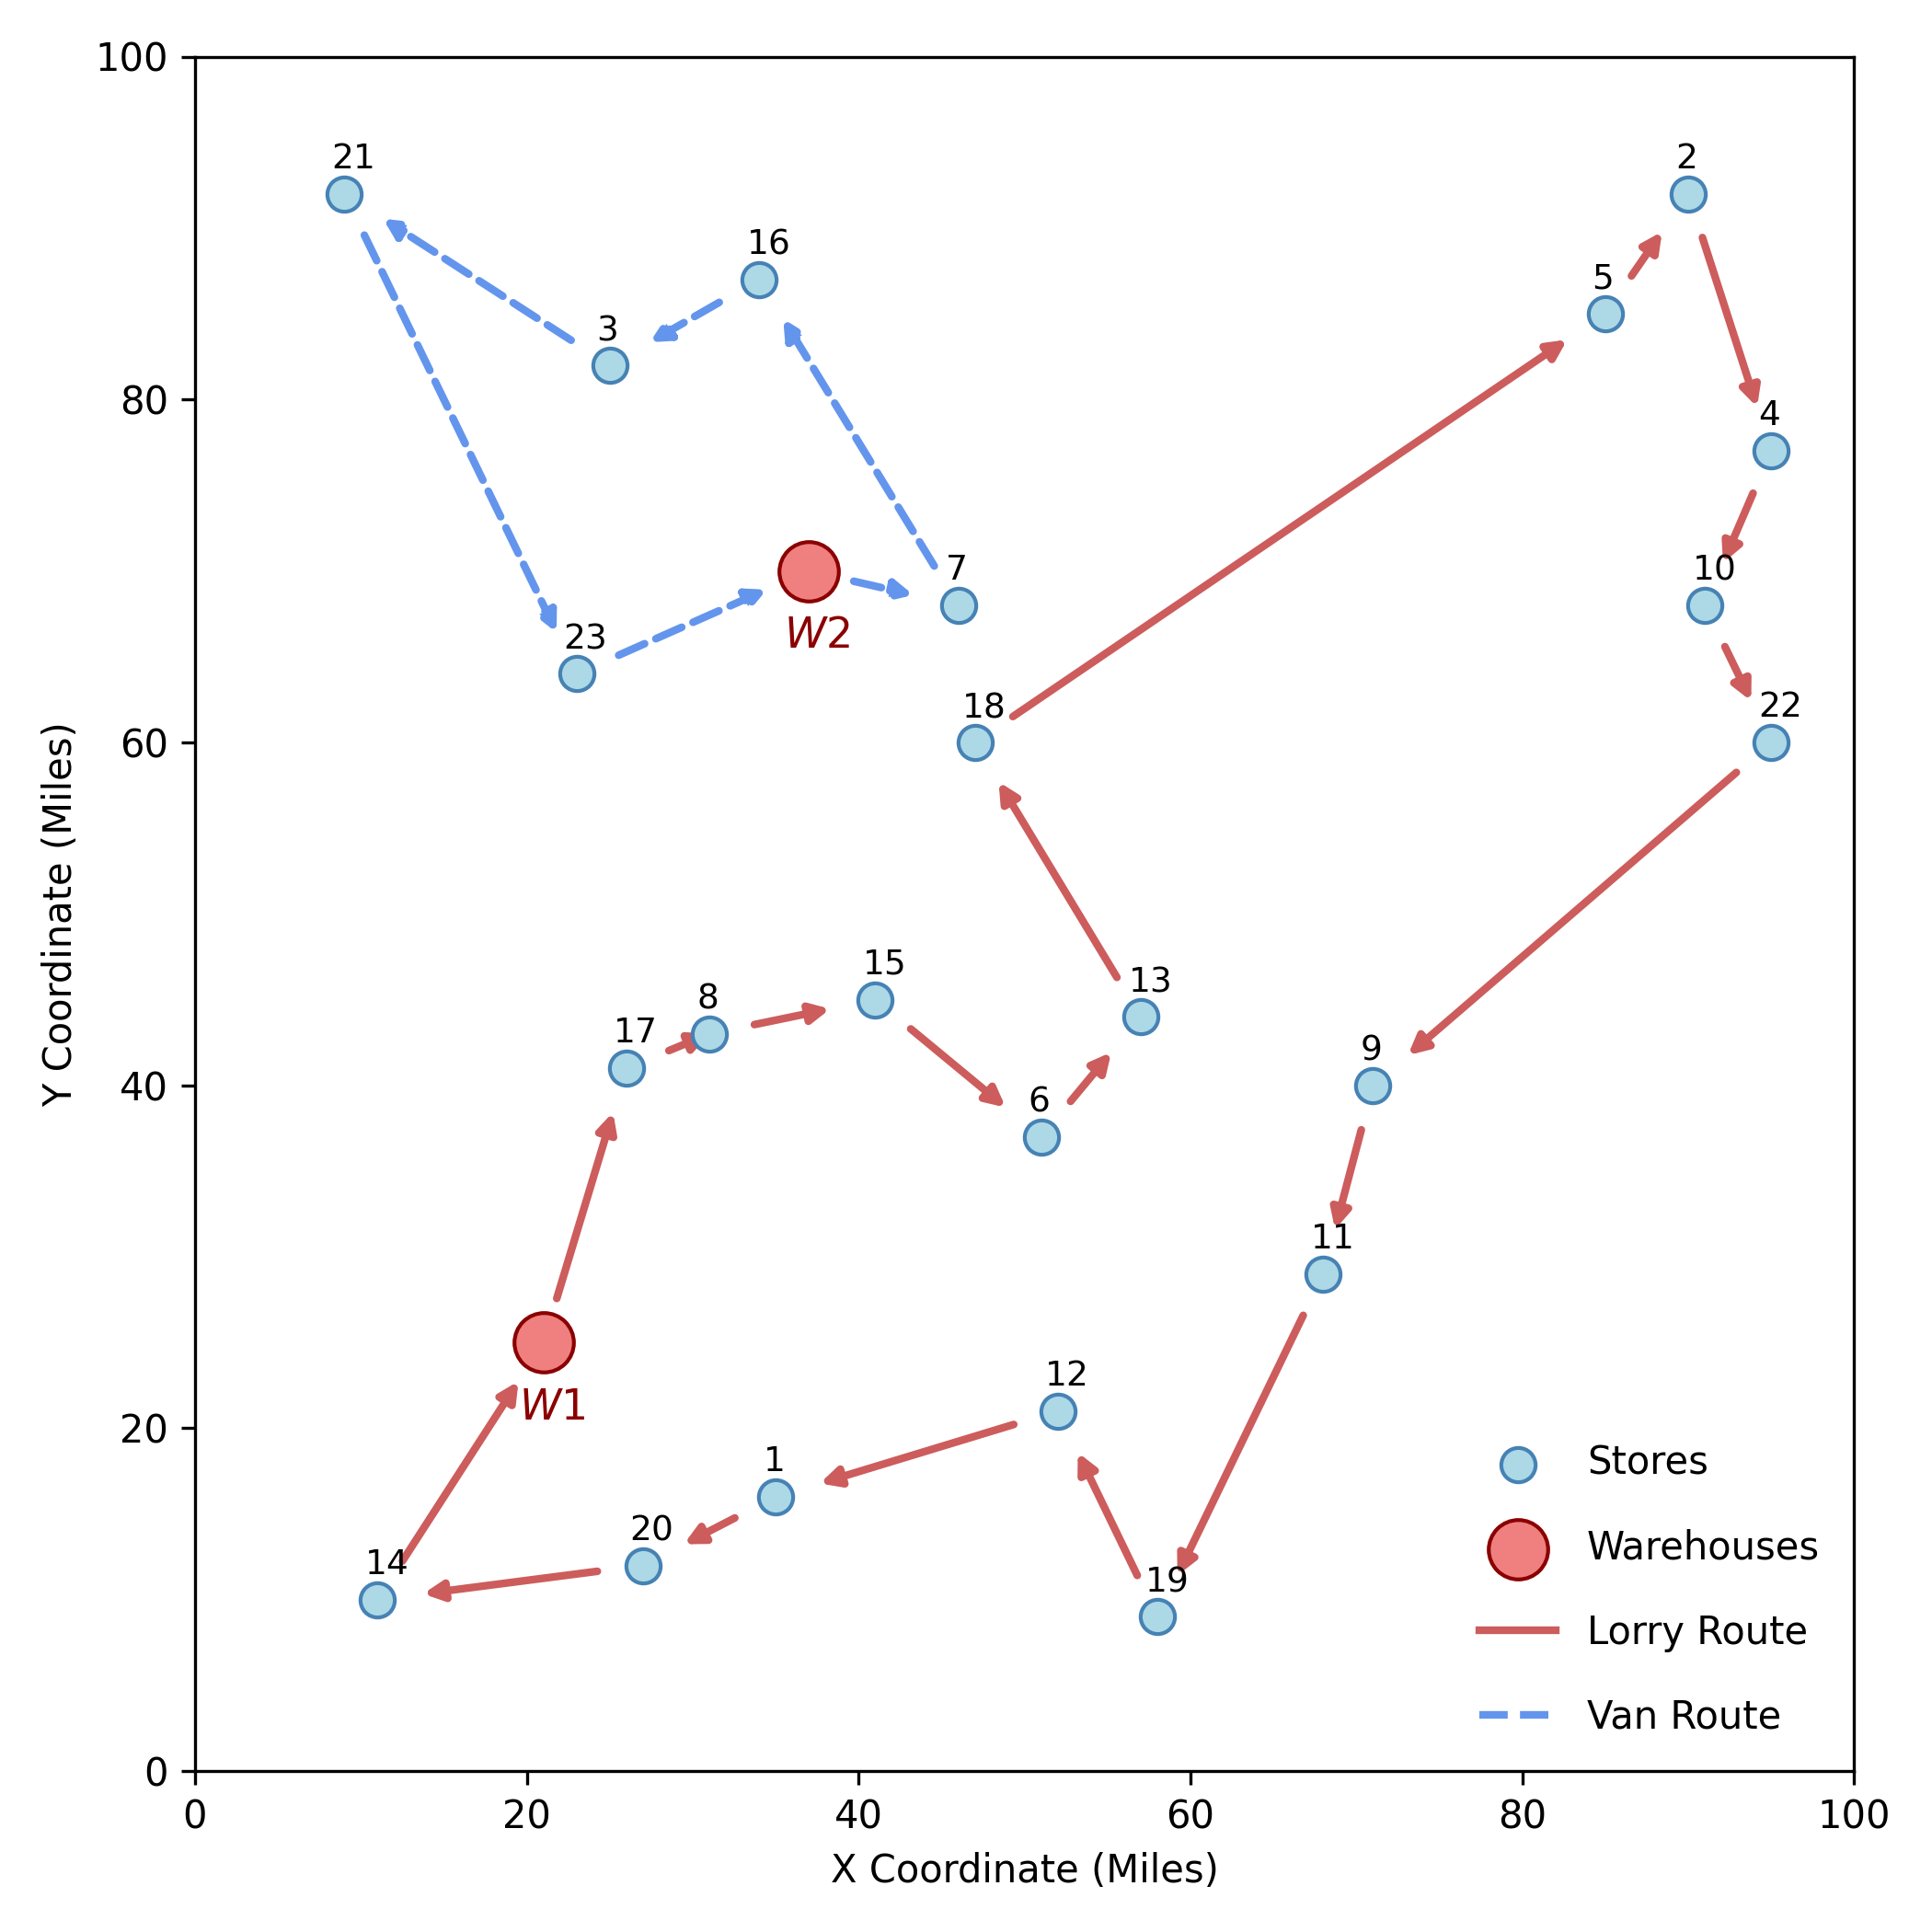
\includegraphics[width=0.85\linewidth]{images/supermarket_final_routes.png}
    \caption{The optimised distribution network. Directional paths denote the $18$-store Lorry route (red) from Warehouse $1$ and the $5$-store Van route (blue) from Warehouse $2$.}
    \label{fig:supermarket_solution}
\end{figure}



\clearpage
\bibliographystyle{ieeetr}
\bibliography{references}

\end{document}